\documentclass[12pt]{report}

\usepackage[english,russian]{babel} 
\usepackage{fontspec} 
\defaultfontfeatures{Ligatures={TeX},Renderer=Basic} 
\setmainfont[Ligatures={TeX,Historic}]{Times New Roman}
\usepackage[utf8]{inputenc}
\usepackage[14pt]{extsizes}
\usepackage{graphicx}
\usepackage{geometry}
\usepackage{listings}
\usepackage{fontspec} 

% Для измененных титулов глав:
\usepackage{titlesec, blindtext, color} % подключаем нужные пакеты
\usepackage{setspace} % полуторный интервал
\definecolor{gray75}{gray}{0.75} % определяем цвет
\newcommand{\hsp}{\hspace{20pt}} % длина линии в 20pt
% titleformat определяет стиль
\titleformat{\chapter}[hang]{\Huge\bfseries}{\thechapter\hsp\textcolor{gray75}{|}\hsp}{0pt}{\Huge\bfseries}
\usepackage{caption} % подписи к рисункам в русской типографской традиции

\geometry{top=2cm} % отступ сверху
\geometry{bottom=2cm} % отступ снизу
\geometry{left=3cm} % отступ справа
\geometry{right=1cm} % отступ слева


 \captionsetup[figure]{labelsep=endash,justification=centering,singlelinecheck=false,font=normalsize}

% Для листинга кода:
\lstset{ %
	language=c++,                 % выбор языка для подсветки (здесь это С)
	basicstyle=\small\sffamily, % размер и начертание шрифта для подсветки кода
	numbers=left,               % где поставить нумерацию строк (слева\справа)
	numberstyle=\tiny,           % размер шрифта для номеров строк
	stepnumber=1,                   % размер шага между двумя номерами строк
	numbersep=5pt,                % как далеко отстоят номера строк от подсвечиваемого кода
	showspaces=false,            % показывать или нет пробелы специальными отступами
	showstringspaces=false,      % показывать или нет пробелы в строках
	showtabs=false,             % показывать или нет табуляцию в строках
	frame=single,              % рисовать рамку вокруг кода
	tabsize=2,                 % размер табуляции по умолчанию равен 2 пробелам
	captionpos=t,              % позиция заголовка вверху [t] или внизу [b] 
	breaklines=true,           % автоматически переносить строки (да\нет)
	breakatwhitespace=false, % переносить строки только если есть пробел
	escapeinside={\#*}{*)}   % если нужно добавить комментарии в коде
}


%для графиков
\usepackage{pgfplots}
\usepackage{filecontents}
\usetikzlibrary{datavisualization}
\usetikzlibrary{datavisualization.formats.functions}
\begin{filecontents}{LevTable.dat}
	5 80
	10 120
	50 760
	100 2500
	200 9500
	500 55000
\end{filecontents}

\begin{filecontents}{LevRec.dat}
	5 370
	10 1610000
\end{filecontents}

\begin{filecontents}{LevRecTable.dat}
	5 100
	10 150
	50 1680
	100 6700
	200 25000
	500 160000
\end{filecontents}

\begin{filecontents}{DamLevTable.dat}
	5 80
	10 120
	50 860
	100 2900
	200 11000
	500 65000
\end{filecontents}



\begin{document}	
	%\def\chaptername{} % убирает "Глава"
	\begin{titlepage}
		\newgeometry{pdftex, left=2cm, right=2cm, top=2.5cm, bottom=2.5cm}
		\fontsize{12pt}{12pt}\selectfont
		\noindent \begin{minipage}{0.15\textwidth}
			
\includegraphics[width=\linewidth]{baum.jpg}
		\end{minipage}
		\noindent\begin{minipage}{0.9\textwidth}\centering
			\textbf{Министерство науки и высшего образования Российской Федерации}\\
			\textbf{Федеральное государственное бюджетное образовательное учреждение высшего образования}\\
			\textbf{«Московский государственный технический университет имени Н.Э.~Баумана}\\
			\textbf{(национальный исследовательский университет)»}\\
			\textbf{(МГТУ им. Н.Э.~Баумана)}
		\end{minipage}
		
		\noindent\rule{18cm}{3pt}
		\newline\newline
		\noindent ФАКУЛЬТЕТ \underline{«Информатика и системы управления»} 
		\newline\newline
		\noindent КАФЕДРА \underline{«Программное обеспечение ЭВМ и информационные технологии»}
		\newline\newline\newline\newline\newline\newline\newline
		
		
		\begin{center}
			\Large\textbf{Отчет по лабораторной работе №1 \newline по курсу "Анализ алгоритмов"}\newline
		\end{center}
		
		\noindent\textbf{Тема} \underline{Расстояния Левенштейна и Дамерау-Левенштейна}
		\newline\newline\newline
		\noindent\textbf{Студент} \underline{Сусликов Д.В.~~~~~~~~~~~~~~~~~~~~~~~~~~~~~~~~~~~~~}
		\newline\newline
		\noindent\textbf{Группа} \underline{ИУ7-55~~~~~~~~~~~~~~~~~~~~~~~~~~~~~~~~~~~~~~~~~~~~~~~~~~~~~~~~~~}
		\newline\newline
		\noindent\textbf{Оценка (баллы)} \underline{~~~~~~~~~~~~~~~~~~~~~~~~~~~~~~~~~~~~~~~~~~~~~~~~~~~~~~~}
		\newline\newline
		\noindent\textbf{Преподаватели} \underline{Волкова Л.Л., Строганов Ю.В.~~~~~~~~~~~~~~}
		\newline
		
		\begin{center}
			\vfill
			Москва~---~\the\year
			~г.
		\end{center}
		\restoregeometry
	\end{titlepage}
	
	\tableofcontents
	\onehalfspacing
	
	\newpage
	\chapter*{Введение}
	\addcontentsline{toc}{chapter}{Введение}
	
	\textbf{Редакионное расстояние} или \textbf{расстояние Левенштейна} - это минимальное количество редакторских операций, которые необходимо для преобразования одной строки в другую.
	
	Расстояние Левенштейна и его обобщения активно применяется: 
	\begin{itemize}
		\item для автозамен ошибок в слове (например, в поисковых системах);
		\item в биоинформатике для сравнения генов, хромосом и белков;
		\item и в других областях.
	\end{itemize}
	
	Целью данной лабораторной работы:реализовать и сравнить по эффективности алгоритмы поиска расстояний Левенштейна и Дамерау-Левенштейна.
	
	Задачи:
	\begin{enumerate}
		\item Дать математическое описание расстояний Левенштейна и Дамерау-Левенштейна;
		\item Разработать алгоритмы поиска расстояний;
		\item Реализовать алгоритмы поиска расстояний;
		\item Провести эксперименты по замеру времени работы реализации алгоритмов;
		\item Провести сравнительный анализ реализаций алгоритмов по затрачиваемому времени (и максимально затрачиваемой памяти);
		\item Дать теоретическую оценку максимально затрачиваемых по памяти реализациям алгоритмов.
	\end{enumerate}
	
	\chapter{Аналитическая часть} 
	Задачей алгоритма Левештейна является нахождение минимального количества редакционных операций (вставок, удалений, замен) нужных для приведения одной строки символов к другой.
	
	При нахождении расстояния Дамерау—Левенштейна добавляется операция перестановки двух соседних символов. 
	
	\textbf{Действия обозначаются так:} 
	\begin{itemize}
		\item D (delete) — удалить;
		\item I (insert) — вставить;
		\item R (replace) — заменить;
		\item M (match) - совпадение;
		\item X (exchange) - перестановка (только в алгоритме Дамерау—Левенштейна).
	\end{itemize}
Каждая операция, кроме перестановки, увеличивает релакционное расстояние на 1.


Пусть $S_{1}$ и $S_{2}$ — две строки (длиной $i$ и $j$ соответственно) над некоторым алфавитом, тогда расстояние Левенштейна можно подсчитать по следующей рекуррентной формуле:


\begin{equation}
	D(i,j) = \left\{ \begin{array}{ll}
		0, & \textrm{$i = 0, j = 0$}\\
		i, & \textrm{$j = 0, i > 0$}\\
		j, & \textrm{$i = 0, j > 0$}\\
		min(D(S_{1}[1..i],S_{2}[1..j-1])+1,\\
		D(S_{1}[1..i-1],S_{2}[1..j]) +1, &\textrm{$j>0, i>0$}\\
		D(S_{1}[1..i-1],S_{2}[1..j-1]) + m(S_{1}[i], S_{2}[j]))
	\end{array}\right.
\end{equation}

где $m(a,b)$ равно 0 при $a=b$, и 1 в противном случае;

 $min\{\,a,b,c\}$ возвращает наименьший из аргументов.


Расстояние Дамерау-Левенштейна вычисляется по следующей рекуррентной формуле:

\begin{equation}
	D(i,j) = \left\{ \begin{array}{ll}
		0, & \textrm{$i = 0, j = 0$}\\
		i, & \textrm{$j = 0, i > 0$}\\
		j, & \textrm{$i = 0, j > 0$}\\
		min(D(S_{1}[1..i],S_{2}[1..j-1])+1,\\
		D(S_{1}[1..i-1],S_{2}[1..j]) +1, &\textrm{$j>0, i>0$}\\
		D(S_{1}[1..i-1],S_{2}[1..j-1]) + m(S_{1}[i], S_{2}[j]))\\
		D(S_{1}[1..i-2],S_{2}[1..j-2]) + 1
	\end{array}\right.
\end{equation}
	
	\chapter{Конструкторская часть}
Далее будут представлены схемы алгоритмов нахождения редакционного расстояния. 

\newgeometry{pdftex, left=2cm, right=2cm, top=2.5cm, bottom=2.5cm}


\section{Разработка алгоритмов}
Ниже на Рисунке 1 представлена схема матричного алгоритма нахождения расстояний Левенштейна.
\begin{figure}[h!]
	\center{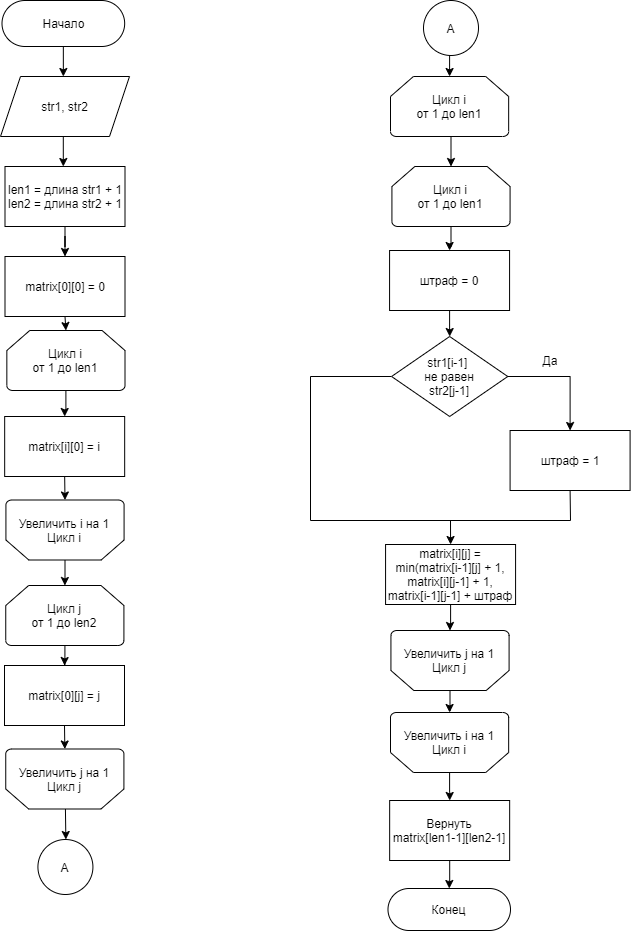
\includegraphics[scale=0.5]{aa1Matrix.png}}
	\caption*{Рисунок 1 - Схема матричного алгоритма Левенштейна}
\end{figure}

\restoregeometry

\newpage
Далее на Рисунке 2 можно увидеть схему рекурсивного алгоритма нахождения расстояния Левенштейна.
\begin{figure}[h!]
	\center{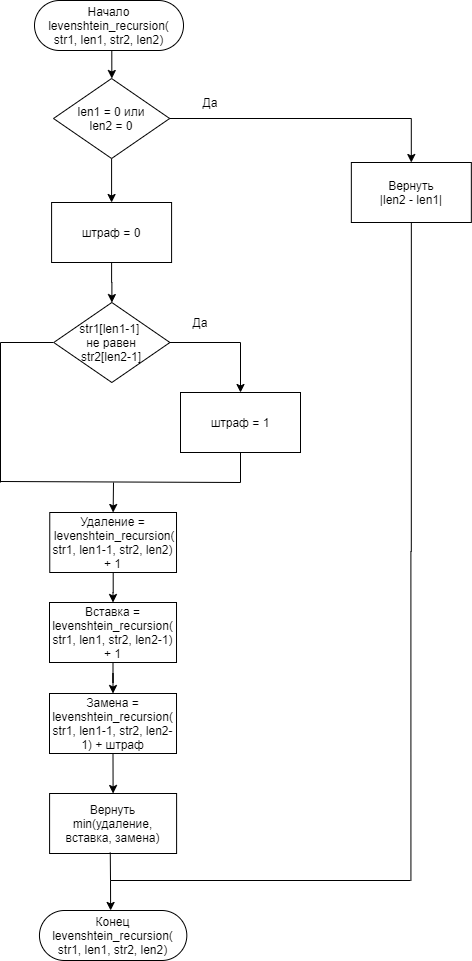
\includegraphics[scale=0.6]{LevRecV2.png}}
	\caption*{Рисунок 2 - Схема рекурсивного алгоритма Левенштейна}
\end{figure}

\newpage
Ниже на Рисунке 3 изображена схема рекурсивного алгоритма с использованием матрицы для нахождения расстояний Левенштейна.
\begin{figure}[h!]
	\center{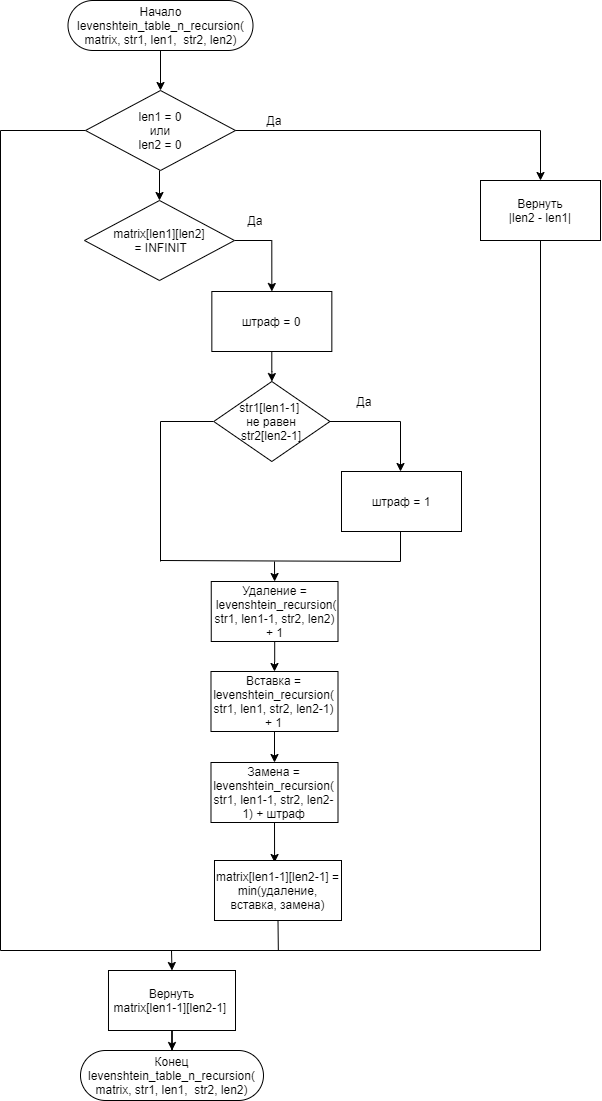
\includegraphics[scale=0.5]{LevRecMatr.png}}
	\caption*{Рисунок 3 - Схема рекурсивного алгоритма Левенштейна с использованием матрицы}
\end{figure}

\newpage
Далее на Рисунке 4 показана схема матричного алгоритма нахождения расстояния Дамерау-Левенштейна.
\begin{figure}[h!]
	\center{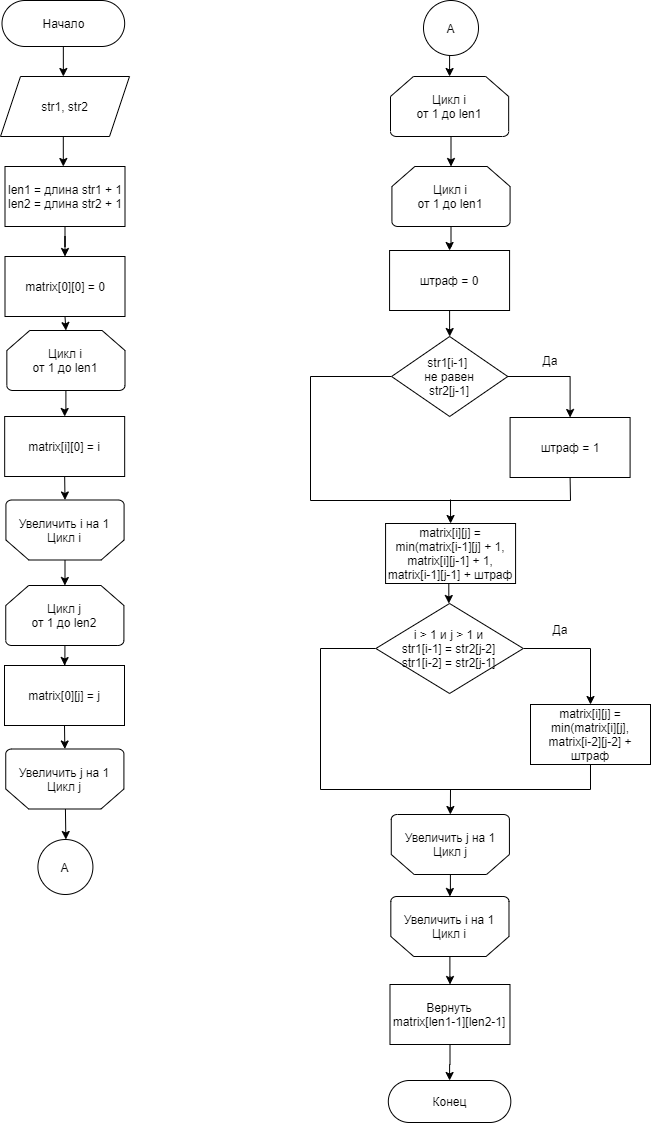
\includegraphics[scale=0.5]{DamerauLev.png}}
	\caption*{Рисунок 4 - Схема матричного алгоритма Дамерау-Левенштейна}
\end{figure}

\section{Сравнительный анализ памяти}
В случае матричной реализации алгоритма, требуется хранить
\begin{itemize}
	\item динамическую матрицу размером $C_1$ * (len1 + 1) + (len1 + 1) * $C_1$ * (len2 + 1),
	\item значения двух счетчиков 2$C_2$,
	\item значение вспомогательной переменной (штраф) $C_2$
\end{itemize}
и передавать параметры ($C_2$ * len).

В итоге, так будет высчитываться общий размер запрашиваемой памяти:
$$C_1 * (len1 + 1) + (len1 + 1) * C_1 * (len2 + 1) + 2C_2 + C_2 * len $$

В случае рекурсивной реализации при каждом вызове требуется хранить значение 4 вспомогательных переменных - 4$C_2$ 
и передавать параметры ($C_2$ * len).

Причем, максимальная глубина рекурсивного вызова – максимальная длина двух строк.

Так как память рекурсивного алгоритма растет пропорционально сумме длин строк, а
матричного – их произведения, то на строках большой длины рекурсивный алгоритм затрачивает меньше памяти по сравнению с матричным.

\chapter{Технологическая часть}
В данном разделе рассматривается выбранный язык программирования, среда разработки, требуемые
инструменты для реализации и сама реализация.


\section{Требования к программному обеспечению}
\begin{enumerate}
	\item Программа должна предусматривать ввод двух строк произвольной длины. Строки
	могут содержать произвольный набор символов.
	\item Выбор применяемого алгоритма осуществляется пользователем из списка алгоритмов,
	предложенных в меню.
	\item На выходе программа выводит матрицу (в случае выбора матричного алгоритма) и
	значение расстояния между введенными строками.
	\item Также необходимо предусмотреть выполнение замеров процессорного времени для
	каждого из алгоритмов.

\end{enumerate}

\section{Средства реализации}
В лабораторной работе быть использован язык $C$++, так как был ранее изучен и использован во многих предыдущих работах.

Среда разработки - $Qt$.

Для замеров процессорного времени была использована функция $clock()$.
\newpage

\section{Реализация алгоритмов}
Листинг 1 - Функция нахождения расстояния матричного алгоритма Левенштейна
\begin{lstlisting}
long int levenshtein_distance(const char* str1, const char* str2)
{
	long int len1 = strlen(str1) + 1;
	long int len2 = strlen(str2) + 1;
	
	int** matrix = create_matrix(len1, len2);
	
	matrix[0][0] = 0;
	for (long int i = 1; i < len1; i++)
		matrix[i][0] = i;
	
	for (long int j = 1; j < len2; j++)
		matrix[0][j] = j;
	
	for (long int i = 1; i < len1; i++)
	{
		for (long int j = 1; j < len2; j++)
		{
			int sub_cost = 0;
			if (str1[i - 1] != str2[j - 1])
				sub_cost = 1;
			
			matrix[i][j] = my_min(matrix[i - 1][j] + DELETION_COST,    
			matrix[i][j - 1] + INSERTION_COST,   
			matrix[i - 1][j - 1] + sub_cost);	
		}
	}	
	int answer = matrix[len1 - 1][len2 - 1];	
	
	print_matrix(matrix, len1, len2);
	free_matrix(&matrix, len1);	
	return  answer;
}
\end{lstlisting}
\newpage

Листинг 2 - Функция рекурсивного алгоритма нахождения расстояний Левенштейна

\begin{lstlisting}
long int levenshtein_recursion(const char* str1, long int len1, const char* str2, long int len2)
{
	if (len1 <= 0 || len2 <= 0)
		return abs((int)(len2 - len1));
	
	int sub_cost = 0;
	if (str1[len1 - 1] != str2[len2 - 1])
		sub_cost = 1;
	
	long int deletion = levenshtein_recursion(str1, len1 - 1, str2, len2) + DELETION_COST;
	long int insertion = levenshtein_recursion(str1, len1, str2, len2 - 1) + INSERTION_COST;
	long int replacement = levenshtein_recursion(str1, len1 - 1, str2, len2 - 1) + sub_cost;
	
	return my_min(deletion, insertion, replacement);
}

long int levenshtein_recursion(const char* str1, const char* str2)
{
	long int len1 = strlen(str1);
	long int len2 = strlen(str2);
	
	if (len1 <= 0 || len2 <= 0)
		return abs((int)(len2 - len1));
	
	int sub_cost = 0;
	if (str1[len1 - 1] != str2[len2 - 1])
		sub_cost = 1;
	
	long int deletion = levenshtein_recursion(str1, len1 - 1, str2, len2) + DELETION_COST;
	long int insertion = levenshtein_recursion(str1, len1, str2, len2 - 1) + INSERTION_COST;
	long int replacement = levenshtein_recursion(str1, len1 - 1, str2, len2 - 1) + sub_cost;
	
	return my_min(deletion, insertion, replacement);
}
\end{lstlisting}

Листинг 3 - Функция рекурсивного алгоритма с использованием матрицы нахождения расстояний Левенштейна

\begin{lstlisting}
long int levenshtein_table_n_recursion(int** matrix, const char* str1,
long int len1, const char* str2, long int len2)
{
	if (len1 <= 0 || len2 <= 0)
		return abs((int)(len2 - len1));
	
	if (matrix[len1][len2] == INFINIT)
	{
		int sub_cost = 0;
		if (str1[len1 - 1] != str2[len2 - 1])
			sub_cost = 1;
		
		long int deletion = levenshtein_table_n_recursion(matrix, str1, len1 - 1, str2, len2) + DELETION_COST;
		long int insertion = levenshtein_table_n_recursion(matrix, str1, len1, str2, len2 - 1) + INSERTION_COST;
		long int replacement = levenshtein_table_n_recursion(matrix, str1, len1 - 1, str2, len2 - 1) + sub_cost;
		
		matrix[len1][len2] = my_min(deletion, insertion, replacement);
	}
	
	return matrix[len1][len2];
}

long int levenshtein_table_n_recursion(const char* str1, const char* str2)
{
	long int len1 = strlen(str1) + 1;
	long int len2 = strlen(str2) + 1;
	
	int** matrix = (int**)create_matrix(len1, len2);
	
	fill_matrix_with_infinity(matrix, len1, len2);
	
	matrix[0][0] = 0;
	for (long int i = 1; i < len1; i++)
	matrix[i][0] = i;
	
	for (long int j = 1; j < len2; j++)
	matrix[0][j] = j;
	
	len1--; len2--;
	
	int sub_cost = 0;
	if (str1[len1 - 1] != str2[len2 - 1])
	sub_cost = 1;
	
	long int deletion = levenshtein_table_n_recursion(matrix, str1, len1 - 1, str2, len2) + DELETION_COST;
	long int insertion = levenshtein_table_n_recursion(matrix, str1, len1, str2, len2 - 1) + INSERTION_COST;
	long int replacement = levenshtein_table_n_recursion(matrix, str1, len1 - 1, str2, len2 - 1) + sub_cost;
	
	int answer = my_min(deletion, insertion, replacement);
	
	print_matrix(matrix, len1, len2);

	free_matrix(&matrix, len1);
	return  answer;
}
\end{lstlisting}


Листинг 4 - Функция матричного алгоритма нахождения расстояний Дамерау-Левенштейна.

\begin{lstlisting}
	long int damerau_levenshtein_distance(const char* str1, const char* str2)
	{
		long int len1 = strlen(str1) + 1;
		long int len2 = strlen(str2) + 1;

		int** matrix = (int**)create_matrix(len1, len2);
		
		matrix[0][0] = 0;
		for (long int i = 1; i < len1; i++)
		matrix[i][0] = i;
		
		for (long int j = 1; j < len2; j++)
		matrix[0][j] = j;
		
		for (long int i = 1; i < len1; i++)
		{
			for (long int j = 1; j < len2; j++)
			{
				int sub_cost = 0;
				if (str1[i - 1] != str2[j - 1])
				sub_cost = 1;
				
				matrix[i][j] = my_min(matrix[i - 1][j] + DELETION_COST,
				matrix[i][j - 1] + INSERTION_COST,
				matrix[i - 1][j - 1] + sub_cost);
				
				if (i > 1 && j > 1 && str1[i - 1] == str2[j - 2]
				&& str1[i - 2] == str2[j - 1])
				{
					matrix[i][j] = std::min(matrix[i][j], matrix[i - 2][j - 2] + sub_cost);
				}
			}
		}
		
		int answer = matrix[len1 - 1][len2 - 1];
		print_matrix(matrix, len1, len2);		
		free_matrix(&matrix, len1);
		
		return  answer;
	}
\end{lstlisting}

\section{Описание тестирования}
Тестирование осуществляется по принципу «черного ящика».
Для проверки корректности программы необходимо предусмотреть наборы различных тестов,
включающих в себя случаи одной и обеих пустых строк, случаи строки, состоящей из одного
символа, случаи эквивалентных строк.


\chapter{Экспериментальная часть}
В данном разделе будут рассмотрены примеры работы программы, произведено тестирование,
выполнены эксперименты по замеру времени, а также сделан сравнительный анализ
полученных данных.

\section{Примеры работы}
Ниже на Рисунке 5 представлен пример работы программы при выборе матричного алгоритма Левенштейна для строк "кит" и "скат".
\begin{figure}[h!]
	\center{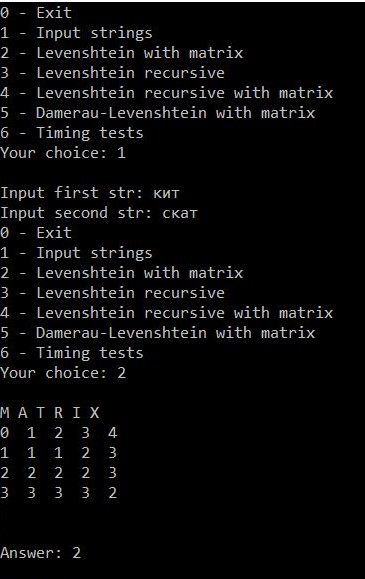
\includegraphics[scale=0.8]{example1.jpg}}
	\caption*{Рисунок 5 - Пример работы программы при выборе матричного алгоритма Левенштейна}
\end{figure}

Ниже на Рисунке 6 представлен пример работы программы при выборе рекурсивного алгоритма Левенштейна для строк "кит" и "скат".
\begin{figure}[h!]
	\center{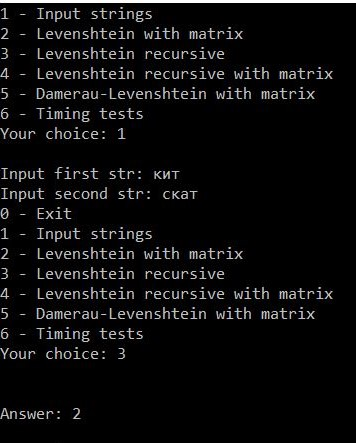
\includegraphics[scale=0.9]{example2.jpg}}
	\caption*{Рисунок 6 - Пример работы программы при выборе рекурсивного алгоритма Левенштейна}
\end{figure}

\newpage
\section{Результаты тестов}
\subsection{Результаты работы программы}

В Таблице 1 показаны результаты работы программы при различных строках. Через "/" показан результат алгоритма Дамерау-Левенштейна в случаях, когда он отличен от результата алгоритма Левенштейна.
\begin{table}[h]
	\caption*{Таблица 1 - Результаты работы программы}
	\begin{center}
		\begin{tabular}{|c c c|}
			\hline
			Первое слово & Второе слово & Результат \\ [0.5ex]
			\hline
			кит & скат & 2\\
			кит & кот & 1\\
			- & - & 0\\
			october & november & 4\\
			123 & 132 & 2 / 1\\
			hotmm & hotmm & 0\\
			\hline
		\end{tabular}
	\end{center}
\end{table}

\subsection{Сравнительный анализ времени работы алгоритмов}
Проведем тестирование по замеру времени работы алгоритмов в зависимости от длины строк. Для этого подсчитаем время работы каждого алгоритма строках длиной 5, 10, 50, 100, 200 и 500 символов. Результаты проведенного эксперимента отображены на Рисунке 7.

%\newpage
\begin{tikzpicture}
	
\begin{axis}[
	axis lines = left,
	xlabel = Длина строки,
	ylabel = {Кол-во тиков},
	legend pos=north east,
	ymajorgrids=true,
	xmajorgrids=true,
	width = 400
]
\addplot[color=red, mark=*] table[x index=0, y index=1] {LevTable.dat}; 
\addplot[color=cyan, mark=*] table[x index=0, y index=1] {LevRec.dat};
\addplot[color=blue, mark=*] table[x index=0, y index=1] {LevRecTable.dat};
\addplot[color=green, mark=*] table[x index=0, y index=1] {DamLevTable.dat};
	
\addlegendentry{LevTable}
\addlegendentry{LevRec}
\addlegendentry{LevRecTable}
\addlegendentry{DamLevTable}
\end{axis}
\end{tikzpicture}

Рисунок 7 - Графики зависимости времени работы алгоритмов от длины строк
\newline\newline
По результатам, отображенным на Рисунке 7, можно сделать вывод, что рекурсивный алгоритм Левенштейна - самый медленный из представленных алгоритмов. Это связано с большим количеством повторных операций. Самым быстрым алгоритмом оказался  матричный алгоритм Левенштейна. Матричный алгоритм Дамерау-Левенштейна работает чуть медленее ранее названного алгоритма из-за операций сравнений, выполняющихся в цикле. Рекурсивный алгоритм Левенштейна с матрицей быстрее рекурсивного, но уступает по скорости выполнения матричным алгоритмам. 

\chapter*{Заключение}
\addcontentsline{toc}{chapter}{Заключение}
В ходе лабораторной работы были разработаны и реализованы алгоритмы нахождения расстояний
Левенштейна (матричный, рекурсивный, рекурсивный с использованием матрицы) и Дамерау-Левенштейна (матричный), а также проведен анализ затрачиваемых ресурсов каждого из метода. По результату анализу стало ясно, что матричные реализации алгоритмов быстрее, чем рекурсивные.

\chapter*{Литература}
\addcontentsline{toc}{chapter}{Литература}

\end{document}



